\documentclass[12pt]{article}
\usepackage[utf8]{inputenc}
\usepackage{chemfig}
\usepackage[version=4]{mhchem}
\usepackage{amsfonts}
\usepackage{amsmath}
\usepackage{amssymb}
\usepackage{geometry}
\usepackage{mathabx}
\usepackage{relsize}
\usepackage{graphics}
\usepackage[colorlinks = true,
            linkcolor = blue,
            urlcolor  = blue,
            citecolor = blue,
            anchorcolor = blue]{hyperref}
%\usepackage{indentfirst}
\usepackage{tikz}
\usepackage{sidecap}
\usepackage{sidecap}
\geometry{
 a4paper,
 total={6.5in,0in},
 left= 15mm,
 top= 15mm,
 bottom=15mm,
 right = 15mm
 }
\title{Methods to Produce Radionuclides with High Energy Efficiency}
\author{Marcos Perez}
\date{June 8 2022 - }

\begin{document}
\maketitle
\section{Simplest Neutron Case: Probability of Zero Interactions}
Consider the following scenario:
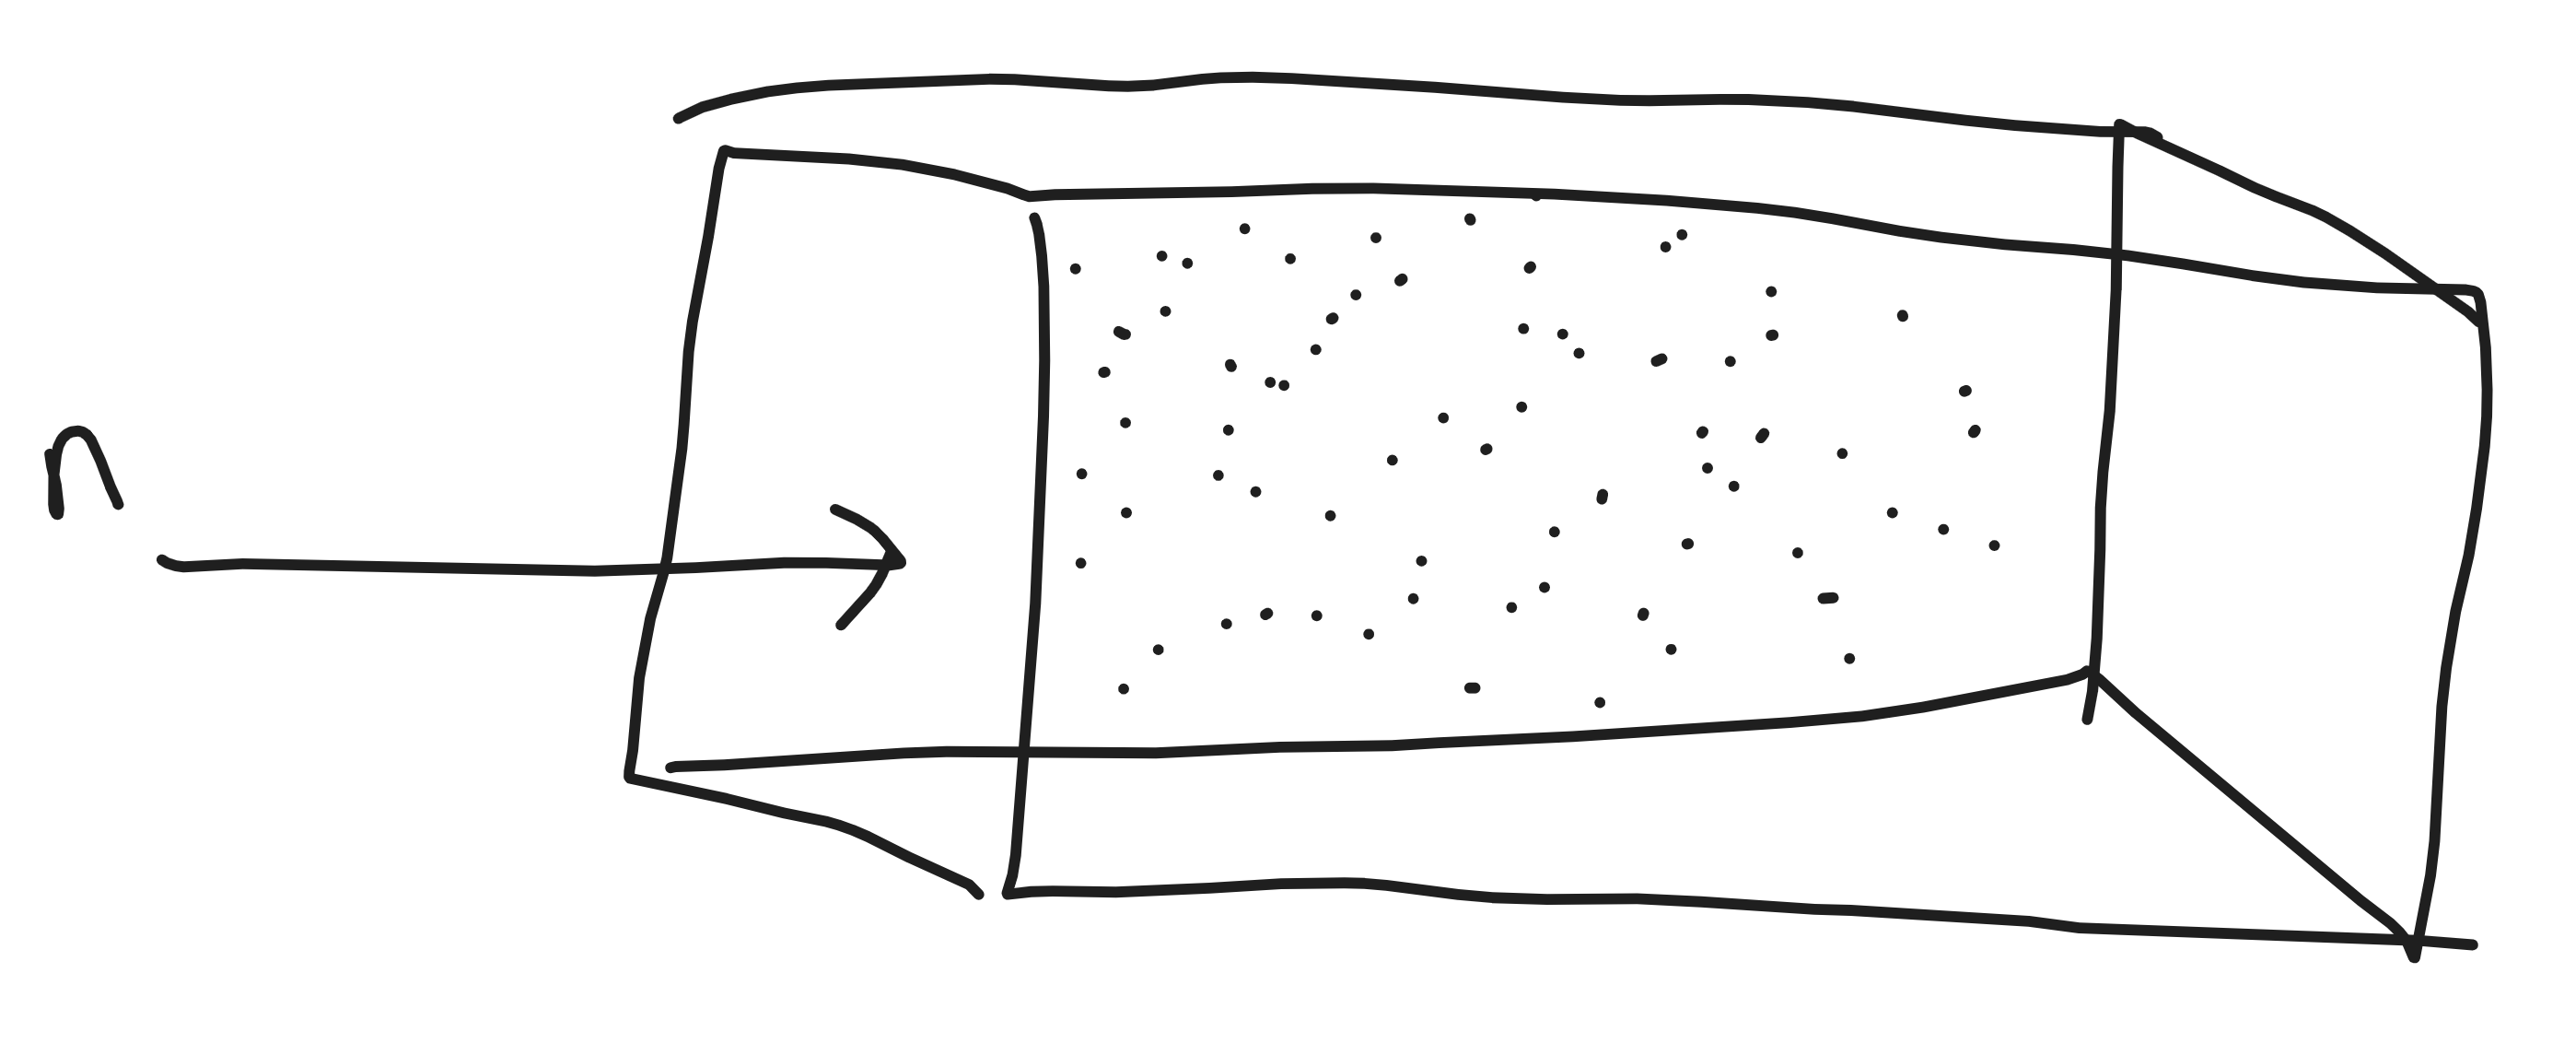
\includegraphics[scale=.4]{Images/simplestCaseNeutron.PNG}\\
A neutron (or anything with negligible stopping power, meaning anything besides a charged particle) enters a homogeneous cloud of particles, each with a cross section $\sigma_E$. Given that unless the neutron collides with a particle, it will continue to travel in a straight line, and if it does not interact with any particles, after travelling $L$ meters through the cloud, it will either decay or escape the cloud. Assuming the neutron is infinitely small, what is the probability of this happening? \\
Assuming there is a probability $P(x,y,z)$ that a given point is within the cross section of a particle. We seek to find the probability that a randomly selected straight line will not intersect the cross section of a particle. Furthermore, the cross section of an individual particle is isotropic. Since the probability that a point $(x,y,z)$ is not within a particle's cross section is $1-P(x,y,z)$. Thus for two points $(x_1,y_1,z_1)$ and $(x_0,y_0,z_0)$ we have for the probability that neither of those points are within the cross section of a particle $(1-P(x_1,y_1,z_1))(1-P(x_0,y_0,z_0)$. Thus for $N$ points we have the probability that there are no cross sections within $N$ points each of the form $x_i,y_i,z_i$
\begin{equation}
\begin{split}
P(n=0) = \prod_{1}^{N} 1-P(x_i,y_i,z_i)
\end{split}
\end{equation}
where $n$ is the number of cross sections within a set of $N$ points in the cloud. 
Using the properties of logarithms then taking the limit as $N\to\infty$ we have
\begin{equation}
\begin{split}
\mathlarger{
P(n=0) = e^{\log(\prod_{1}^{N} 1-P(x_i,y_i,z_i))} = e^{\sum_{1}^{N}\log(1-P(x_i,y_i,z_i))}
}\\
\mathlarger{
\lim_{N\to\infty}P(n=0) = \lim_{N\to\infty} e^{\sum_{1}^{N}\log(1-P(x_i,y_i,z_i))}
}
\end{split}
\end{equation}
Now for the case where the points $(x_i,y_i,z_i)$ are path travelled by the neutron, which we assume to be of the form $(x(t), y(t), z(t))$. Furthermore, since the cross sections are a scalar field we have
\begin{equation}
\begin{split}
\mathlarger{
\lim_{N\to\infty}P(n=0) =  e^{\int_a^b\log(1-P(c(t))\mid c'(t)\mid dt} 
} \\
\end{split}
\end{equation}
where $c(t)$ describes the path of the neutron and its location at a time $t$, where $c(a)$ and $c(b)$ are the two endpoints of the path. Now let us consider the case where $c(t) = (vt, 0, 0)$. Thus we have $\mid c'(t)\mid = v$ which gives
\begin{equation}
\begin{split}
\mathlarger{
\lim_{N\to\infty}P(n=0) =  e^{v\int_a^b\log(1-P((vt, 0, 0))dt} 
} \\
\end{split}
\end{equation}
Now let us assume that the particles within the cloud are uniformly distributed. Thus the cross sections within the cloud have a collective area of
\begin{equation}
\begin{split}
\mathlarger{
A = \frac{\sigma N_AV\rho}{M}
}\\
\end{split}
\end{equation}
where the volume of the cloud is $V$, it has a mass density of $\rho$, $N_A$ is Avogadro's number,s and the molar mass of the particles is $M$. \\
On average, a volume of $v$ in the cloud will contain 1 particle. 
\begin{equation}
\begin{split}
\mathlarger{
N = \frac{N_AV\rho}{M}
}\\
\mathlarger{
v = \frac{V}{N} = \frac{VM}{N_AV\rho} = \frac{M}{N_A\rho}
}\\
\end{split}
\end{equation}
Since we consider the cross section $\sigma$ to be isotropic, consider this volume to be that of a sphere with a particle at its center, then the cross sectional area of that sphere would be 
\begin{equation}
\begin{split}
\mathlarger{
r = \frac{3}{4\pi}v^{\frac{1}{3}} = \frac{3}{4\pi}(\frac{M}{N_A\rho})^{\frac{1}{3}} 
}\\
\mathlarger{
\sigma_{sphere} = \pi r^2 = \pi\frac{9}{16}v^{\frac{2}{3}} = \pi\frac{9}{16}(\frac{M}{N_A\rho})^{\frac{2}{3}}
}\\
\end{split}
\end{equation}
Furthermore, we have for the ratio of the sphere's cross section covered by particle's cross section 
\begin{equation}\label{eqn:isParticleInSphere}
\begin{split}    
\mathlarger{
\frac{\sigma}{\sigma_{sphere}} = \frac{16\sigma}{9\pi v^{\frac{2}{3}}} = 
\frac{16\sigma}{9\pi}(\frac{N_A\rho}{M})^{\frac{2}{3}}
}\\
\end{split}
\end{equation}
Now consider the cloud to be in a rigid box, with the face towards the projectiles is $a\times b$ in terms of sphere diameters. Thus each cross section would consist of $ab$ spheres. Thus we have for the fraction of the box's cross sectional area covered by the spheres 
\begin{equation}\label{eqn:isSphereInBox}
\begin{split}
\mathlarger{
\frac{ab\sigma_{sphere}}{ab2r} = \frac{\pi}{2} r = \frac{3}{8}(\frac{M}{N_A\rho})^{\frac{1}{3}} 
}\\
\end{split}
\end{equation}
Thus the product of the right sides of Equations \ref{eqn:isParticleInSphere} and \ref{eqn:isSphereInBox} is the fraction $f$ of the total cross sectional area of the box covered by particles in the cloud 
\begin{equation}\label{eqn:isParticleInBox}
\begin{split}
\mathlarger{
f = \frac{2\sigma}{3\pi}(\frac{N_A\rho}{M})^{\frac{1}{3}}
}\\
\end{split}
\end{equation}
Thus for a box with thickness $l$ in terms of sphere radii, the probability of a path not intercepting the cross section of any particles is 
\begin{equation}\label{eqn:isParticleInBox}
\begin{split}
\mathlarger{
(1-f)^l = (1-\frac{2\sigma}{3\pi}(\frac{N_A\rho}{M})^{\frac{1}{3}})^l
}\\
\end{split}
\end{equation}
And thus the probability of the path intercepting the cross section of at least 1 particle.
\begin{equation}\label{eqn:isParticleInBox}
\begin{split}
\mathlarger{
1-(1-f)^l = 1-(1-\frac{2\sigma}{3\pi}(\frac{N_A\rho}{M})^{\frac{1}{3}})^l
}\\
\end{split}
\end{equation}





\end{document}